\newpage
\section{内径5mmの細径軸方向繊維強化型空圧筋の開発}
本研究では液体ラテックスを用いたゴム風船の作成方法をベースに,軸方向繊維強化型空気圧人工筋肉を開発する.
本章ではまず細径なゴム風船を作成し,液体ラテックスの扱いに関するノウハウを得る.それを踏まえて,内径5mmの細径軸方向繊維強化型空圧筋の開発を行う.
\subsection{液体ラテックスについて}
ラテックスは,天然ゴムの一種で,主にゴムの木から得られる液体のこと示す.ラテックスは乳白色の液体であり,
そのままでは非常に粘度が高く,様々な成分が含まれている.ラテックスは,製品化される際に加工され,ゴム製品や医療用の手袋などに使用されている\cite{4}.
今回使用する前加硫ラッテクス PC-518 メーカー:有限会社 ハイラテックは薄い商品(風船,手袋,サックなど)作製に向いている.
使用方法としては,成形したい金型をPC-518液の中にドブ漬け、タレが出来ないようにゆっくり引き上げる.
そのまま放置或いは熱風により乾燥させる\cite{5}.
以降,本稿において特に断らない限り液体ラテックス(液体ゴム)とは「REGITEX 液体ゴム (前加硫ラッテクス)」を,凝固液とは「PC-518用凝固液」を指すものとする
.また液体ラテックスおよび凝固液の乾燥には時間がかかるため,これを短縮するためにドライヤー(図\ref{fig:3})を用いた.
これについても,以降特に断らない限りドライヤーとは「Panasonic EH-Ne13」を指すものとする.
\subsection{細径ゴムの試作}
液体ラテックスの扱いに関するノウハウを得るために,一般的なゴム風船の作成方法\cite{6}を参考に,細径なゴム風船を試作した.
ゴム風船を作成する際には白熱電球状のガラス製の型を用いて,その表面に薄く液体ゴムを纏わせることで薄いゴム膜を形成する.
その手法を踏まえて,直径が5mmの鉄製の細棒にゴムを纏わせることで細径なゴム風船を作成することを試みた.
\subsubsection{作製手順}
図\ref{fig:3}に作製に必要な物品,図\ref{fig:4}に作製手順を示す.必要な物品は以下の通りである.
\begin{itemize}
    \item 鉄棒(内径5 mm,3 mm)
    \item 前加硫ラッテクス PC-518 メーカー:有限会社 ハイラテック
    \item PC-518用 凝固液
    \item ドライヤー Panasonic EH-Ne13
    \item ポリメスシリンダー(PC-518,凝固液用)
  \end{itemize}
  以下,作製手順である.
\begin{enumerate}
    \item まず初めに鉄棒を凝固液に約5秒浸して取り出す
    \item 取り出した鉄棒を凝固液の水滴がなくなるまでドライヤーで乾かす(水滴が残っているとゴムがダマになってしまいゴム厚に偏りが生じ,破裂が起きやすくなるのでよく乾かす)
    \item 鉄棒を液体ゴムに約10秒浸して取り出す(容器に鉄棒が触れるとゴムの外膜が剥がれるので注意する)
    \item 凝固液に約5秒浸して取り出す
    \item 取り出した鉄棒をゴム膜の外側のいろが白色から肌色になるまでドライヤーで乾かす
    \item 3時間程部屋で乾かしたら鉄棒からゴム膜をとる(部屋で放置しすぎるとゴムが硬くなりすぎて鉄棒から取り外すときに割れたり,穴が空きやすくなるので注意する)
\end{enumerate}
以上の手順で作成した細径ゴム風船を図\ref{fig:5}に示す.細径ゴム風船の試作を行うことで,凝固液の適切な乾かし方,液体ゴムに浸す時間について
確認することができた.
\begin{figure}[!h]
  \centering  % 図全体を中央に配置
  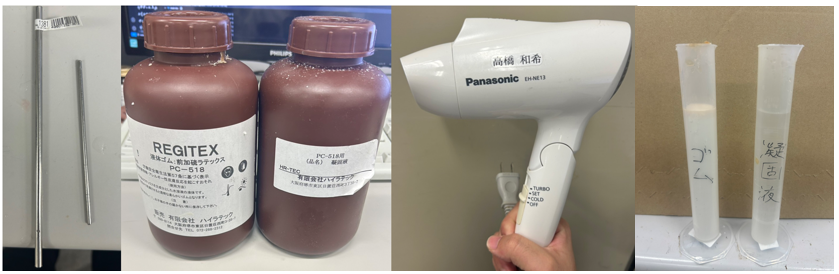
\includegraphics[scale=0.5]{pic/kigu.PNG}
  \caption{使用器具}
  \label{fig:3}
\end{figure}
\begin{figure}[!h]
  \centering  % 図全体を中央に配置
  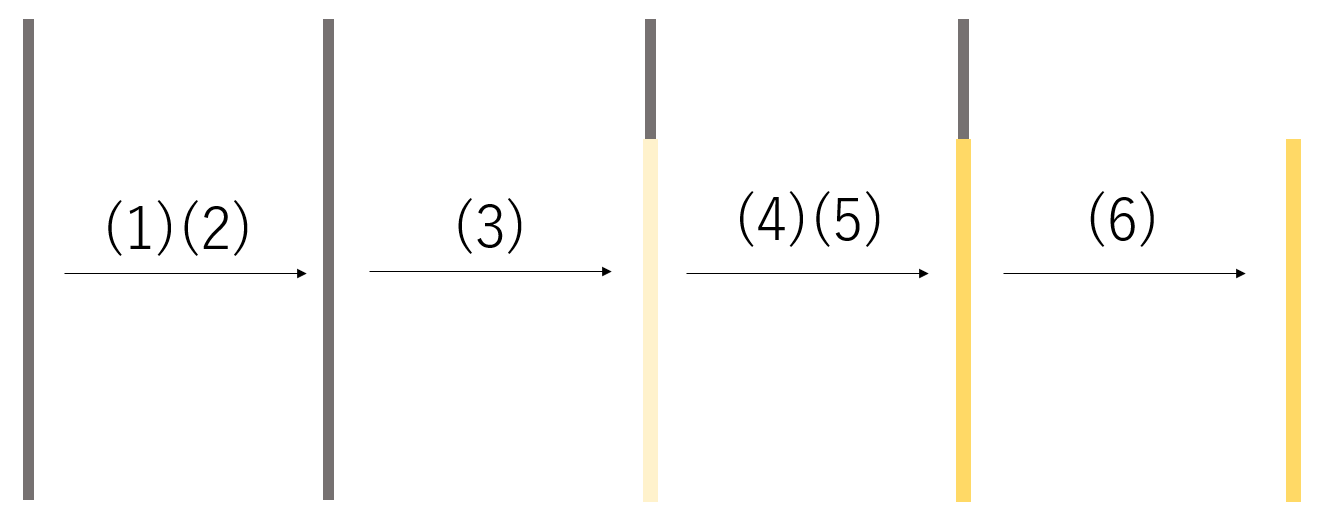
\includegraphics[scale=0.35]{pic/tezyun.PNG}
  \caption{風船の作製手順}
  \label{fig:4}
\end{figure}
\begin{figure}[!t]
  \centering  % 図全体を中央に配置
  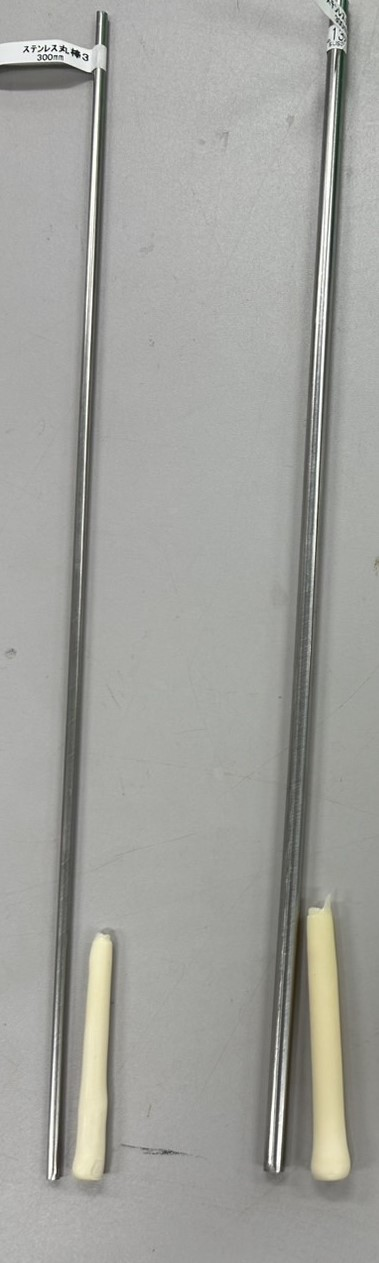
\includegraphics[scale=0.28]{pic/balloon.jpg}
  \caption{作製した風船}
  \label{fig:5}
\end{figure}

\newpage
\subsubsection{問題点の改善}
前項の作製方法で風船を作製するとゴム膜が硬すぎる,ゴム膜の上下で厚さにムラができる問題が生じた.この問題を解決するためにそれぞれ以下のような対策をとった.
まずゴム膜が硬すぎるために膨張させることに必要な印加圧力高く,破裂が起きやすい問題に対して,
液体ゴムを水で割ることで粘度を下げ,膜厚を薄くすることで解決を試みた.前述の通り,液体ゴムの原液を用いて細径風船を作成した場合,
ゴム膜が厚く硬いために破裂してしまった(図\ref{fig:gen}).そこで一般的なゴム風船作製方法を参考にゴム 60: 水 40 の割合で混ぜたものを用いて
細径ゴムの作製を行ったところ\cite{},図\ref{fig:60}のように破裂をすることなく膨張することが確認できた.また実験的
にさらに薄めたゴム 40: 水 60 での割合で混ぜたもので細径ゴム風船の作成を行ったところ,かろうじてゴム膜
を形成することができたが,非常に薄いために空圧を印加するとすぐに膨張が始まり,図\ref{fig:40}のように破裂が生
じてしまった.これらの結果を踏まえて,特に断らない限り以降,作成に用いる液体ゴムはゴム 60: 水 40 の割
合で割ったものを用いることとする.

\begin{figure}[h]
  \centering  % 図全体を中央に配置
  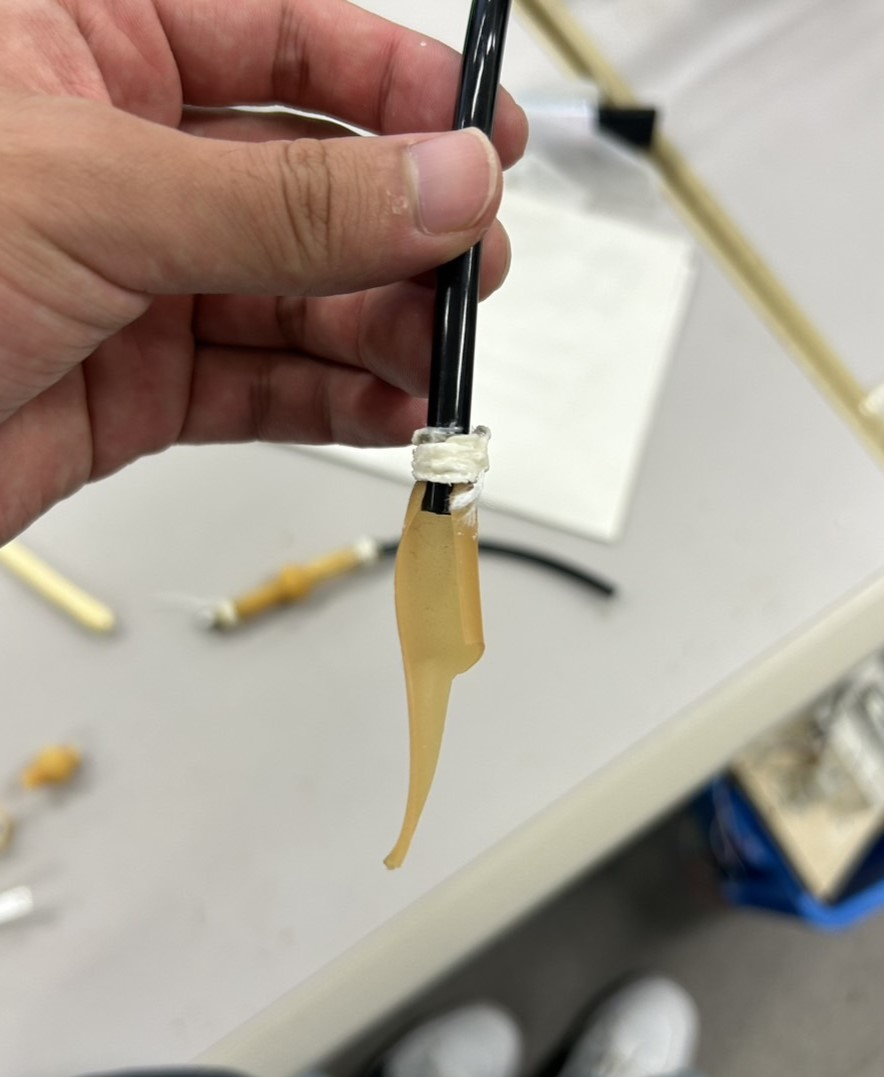
\includegraphics[scale=0.2]{pic/5.jpg}
  \caption{ゴム原液}
  \label{fig:gen}
\end{figure}
\begin{figure}[h]
  \centering
  \begin{minipage}{0.49\hsize}
      \centering
      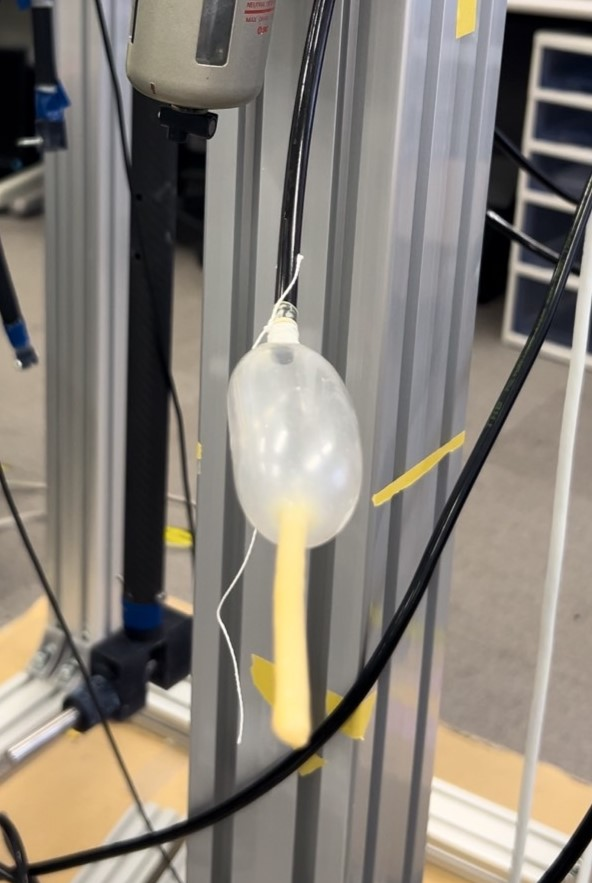
\includegraphics[scale=0.25]{pic/zu6.jpg}
      \caption{ゴム60:水40}
      \label{fig:60}
  \end{minipage} \hfill
  \begin{minipage}{0.49\hsize}
      \centering
      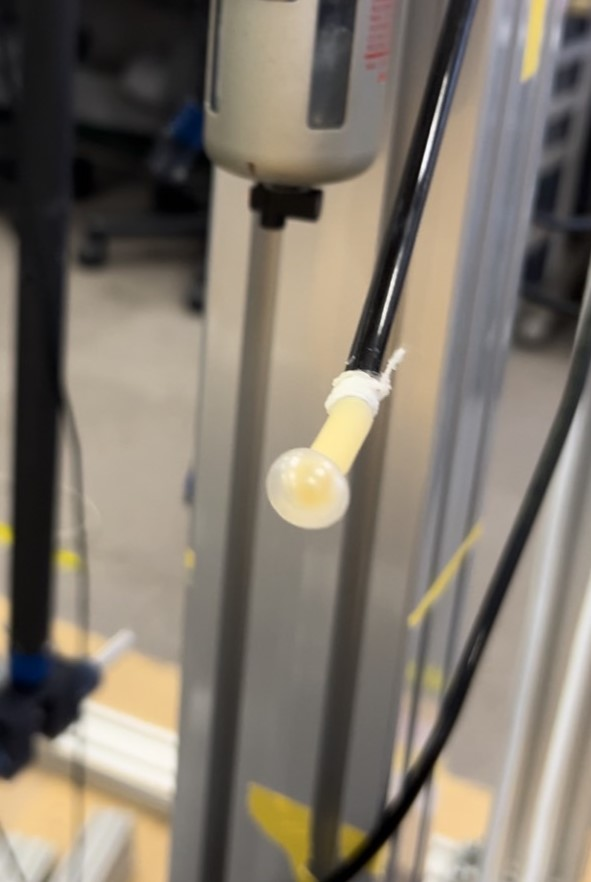
\includegraphics[scale=0.25]{pic/zu5.jpg}
      \caption{ゴム40:水60}
      \label{fig:40}
  \end{minipage} 
\end{figure}
\newpage
次にゴムの上下で厚さに差が出ている問題に対して作製方法の変更で解決を試みた.図\ref{fig:4}を見れば分かるように鉄
棒は一度だけ一方向から液体ゴムに浸されている.時間の経過によって液体ゴムは下へ垂れるため,棒の下側部分と中程部分とでは,下側部分の方が厚くなる.そこで1度液体ゴムに漬けたのち,上下をひっくり返してもう1度
ゴムに漬けることでこれを解決した.
作製手順を以下と図\ref{fig:2kai}に示す.
\begin{enumerate}
  \item まず初めに鉄棒を凝固液に約5秒浸して取り出す
  \item 取り出した鉄棒を凝固液の水滴がなくなるまでドライヤーで乾かす
  \item 鉄棒を液体ゴムに約5秒浸して取り出す
  \item ドライヤーで凝固液の水滴がなくなるまで乾かす
  \item 鉄棒を液体ゴムに約5秒浸して取り出す
  \item 凝固液に約5秒浸して取り出す
  \item 取り出した鉄棒をゴム膜の外側のいろが白色から肌色になるまでドライヤーで乾かす
  \item 3時間程部屋で乾かしたら鉄棒からゴム膜をとる
\end{enumerate}
作製した細径ゴム風船を図\ref{fig:huu}に示す.図\ref{fig:huu}のように上下でゴム厚にムラができることなく作製することができた.
\begin{figure}[!h]
  \centering  % 図全体を中央に配置
  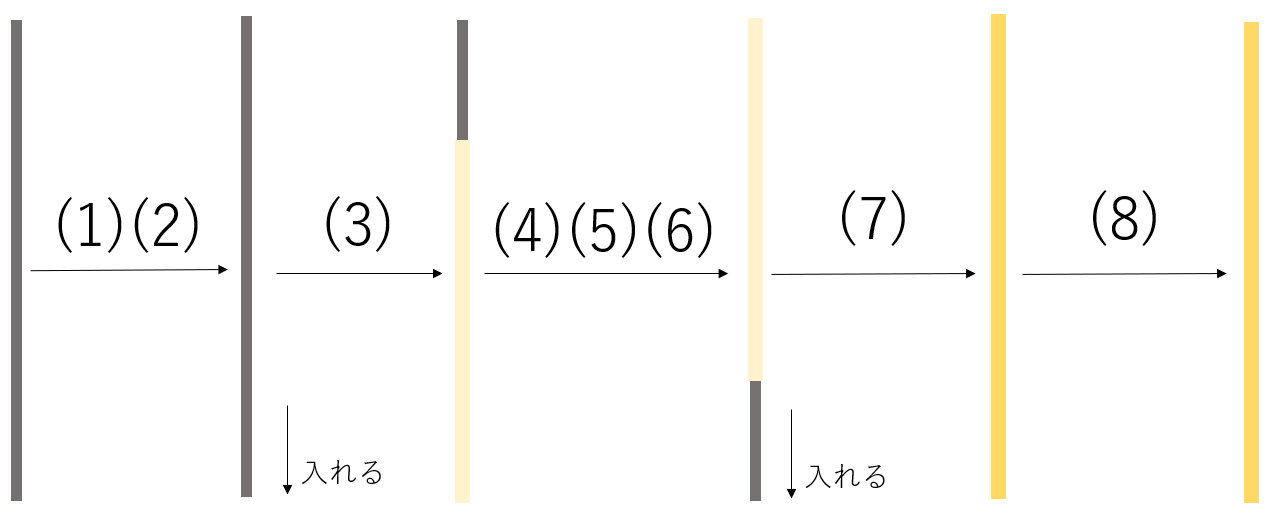
\includegraphics[scale=0.35]{pic/tezyun2.PNG}
  \caption{液体ゴムに上下2回に分けて浸す}
  \label{fig:2kai}
\end{figure}
\begin{figure}[h]
  \centering  % 図全体を中央に配置
  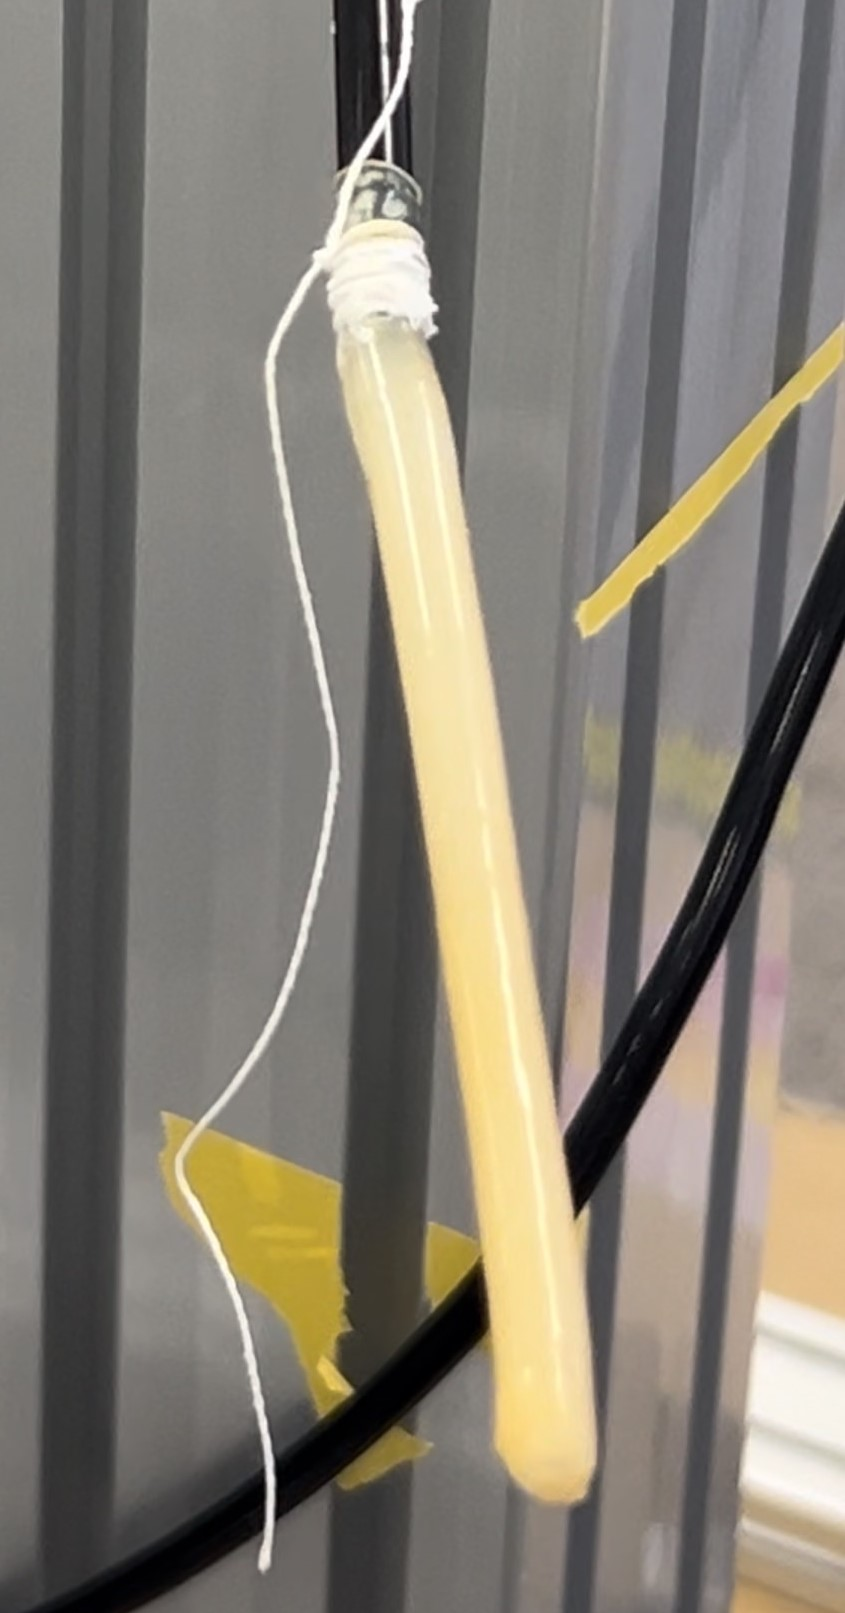
\includegraphics[scale=0.15]{pic/10.jpg}
  \caption{細径ゴム風船}
  \label{fig:huu}
\end{figure}

\newpage

\subsection{内径5 mmの人工筋肉の作製}
前章で細径ゴム風船を作成したノウハウに基づいて,内径5 mmの軸方向繊維強化型細径空圧筋の作製を行った.軸方向繊維強化型の空圧筋を作成するためには,ゴム膜の内
部に繊維(糸)を内包させる必要がある.そこで型である鉄棒の周りに糸を配置するための器具を開発した.
開発した器具の写真を図\ref{fig:11},\ref{fig:12}に示す.
使用方法としては図\ref{fig:13},\ref{fig:14}のように,鉄棒に器具をはめ,糸を通す仕組みになっている.
\begin{figure}[h]
  \centering
  \begin{minipage}{0.49\hsize}
      \centering
      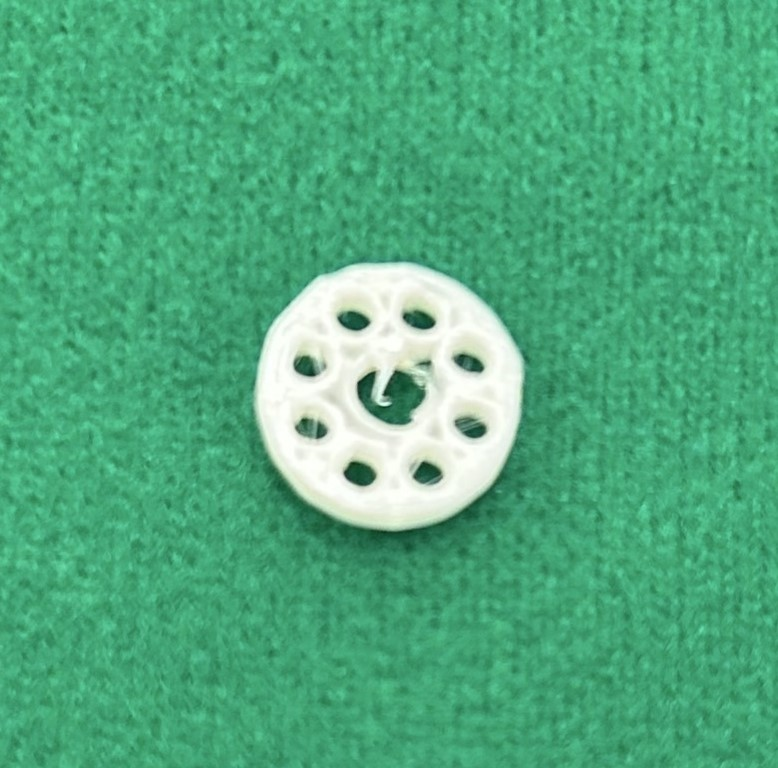
\includegraphics[scale=0.25]{pic/kigu2.jpg}
      \caption{開発した器具}
      \label{fig:11}
  \end{minipage} \hfill
  \begin{minipage}{0.49\hsize}
      \centering
      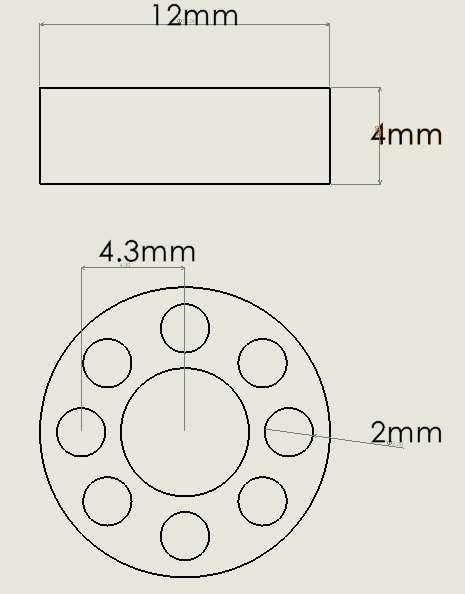
\includegraphics[scale=0.5]{pic/5mm.PNG}
      \caption{開発した器具}
      \label{fig:12}
  \end{minipage} 
\end{figure}

\begin{figure}[h]
  \centering  % 図全体を中央に配置
  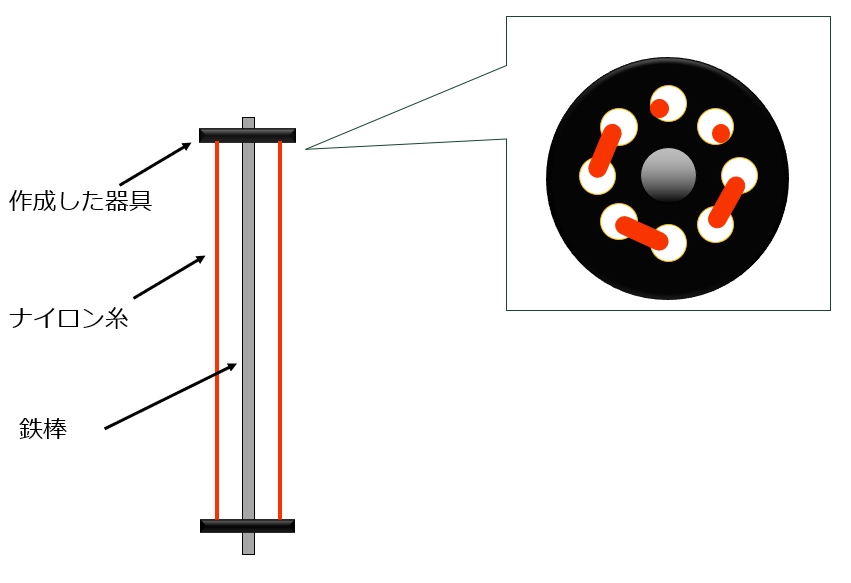
\includegraphics[scale=0.5]{pic/tukau2.PNG}
  \caption{使用方法}
  \label{fig:13}
\end{figure}

\begin{figure}[!h]
  \centering  % 図全体を中央に配置
  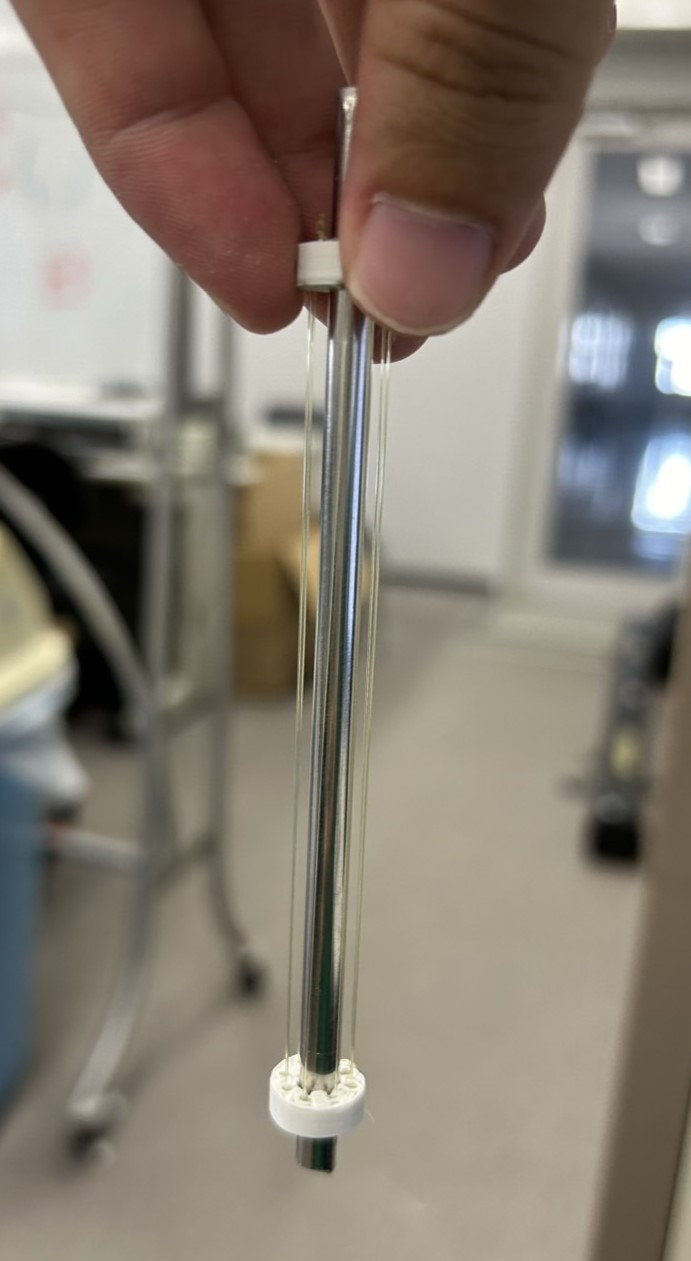
\includegraphics[scale=0.3]{pic/tukau.jpg}
  \caption{使用方法}
  \label{fig:14}
\end{figure}
\newpage
今回は縦糸として3号のナイロン製釣り糸を用いた.図\ref{fig:15}に作製手順を示す.なおここで接着剤とはPPX(セメダイン社,CA-522)を
指す.なお以降特に断らない限り接着剤とはこれを指すものとする.
\begin{itemize}
  \item 鉄棒(内径5 mm)
  \item REGITEX 液体ゴム(前加硫ラッテクス) メーカー:有限会社 ハイラテック
  \item PC-518用 凝固液
  \item ドライヤー Panasonic EH-Ne13
  \item ポリメスシリンダー(PC-518,凝固液用)
  \item 道糸ナイロン 3号 200 m
  \item PPX(瞬間接着剤) メーカー:セメダイン品番:CA-522
  \item PEライン 0.04 mm
\end{itemize}
作製手順を以下に示す.
\begin{enumerate}
  \item まず初めに上記に述べた器具を鉄棒に取り付ける(固定できない場合は接着剤を少し塗り,固定する)
  \item ナイロン糸(3号)を器具に通す
  \item 凝固液に約5秒浸して取り出す
  \item 凝固液の水滴がなくなるまでドライヤーで乾かす
  \item 液体ゴムに約5秒浸して取り出す
  \item 凝固液に約5秒浸して取り出す
  \item ドライヤーで凝固液の水滴がなくなるまで乾かす
  \item 液体ゴムに約5秒浸して取り出す
  \item 凝固液に約5秒浸して取り出す
  \item 取り出した鉄棒をゴム膜の外側のいろが白色から肌色になるまでドライヤーで乾かす
  \item 3時間程部屋で乾かしたら鉄棒からゴム膜をとる
\end{enumerate}
\begin{figure}[h]
  \centering  % 図全体を中央に配置
  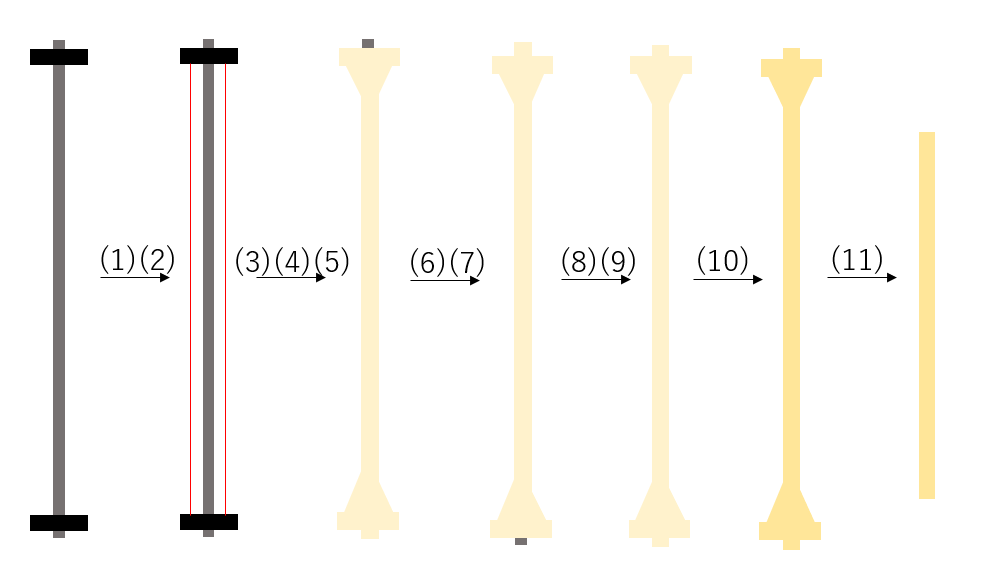
\includegraphics[scale=0.35]{pic/14.PNG}
  \caption{作製手順}
  \label{fig:15}
\end{figure}
上記手順で作成した作成した空圧筋を図\ref{fig:16}に示す.
\begin{figure}[h]
  \centering  % 図全体を中央に配置
  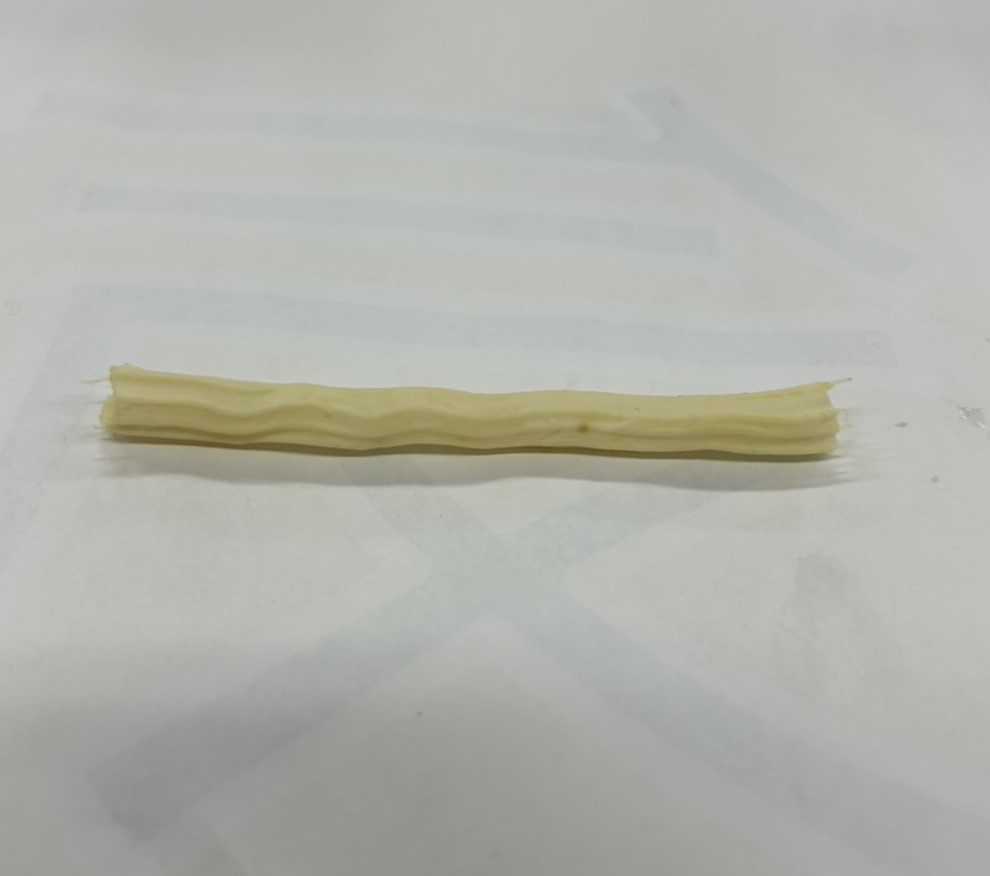
\includegraphics[scale=0.3]{pic/16.jpg}
  \caption{作製した空圧筋}
  \label{fig:16}
\end{figure}
\newpage
作製した繊維内包ゴム被膜を空圧筋として動作させるために図\ref{fig:17}のようにOリング 5mm,M3ネジ,PEライン 0.4 mm,シリコンゴムチューブ 外形 5mmを使用して作製を行った.
作製手順を以下に示す.
\begin{enumerate}
  \item 送気用のポリウレタンチューブを約5 cm切る
  \item 作製した空圧筋をポリウレタンチューブに約1 cm差し込む
  \item 重なった部分をPEラインで結び,強く締結する
  \item 締結下部分に接着剤を塗布し糸が緩まないようにする
  \item Oリングを任意の数はめ込む
  \item M3ネジを他方に挿入して同様にPEラインで締結し,接着剤を塗布することで完成する
\end{enumerate}
\begin{figure}[!h]
  \centering  % 図全体を中央に配置
  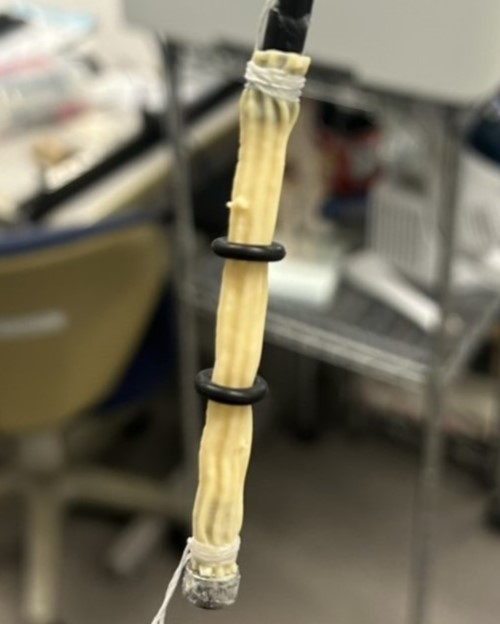
\includegraphics[scale=0.3]{pic/ww.jpg}
  \caption{作製した空圧筋}
  \label{fig:17}
\end{figure}
\newpage

\section{内径3 mmの細径軸方向繊維強化型空圧筋の開発}
前章では,ゴム風船の作製方法を応用することで内径5 mmの人工筋肉の作製に成功した.そこで本章ではさらに細い内径3 mmの人工筋肉の開発に取り組む.
開発においては,前章での手法をベースに試行錯誤を行い,最終的に作製手順5にて作製に成功した.以下に各手法の概略と,その過程で生じた問題点について述べる.
作製するにあたって新しく開発した器具を図\ref{fig:setu}に示す.
\begin{figure}[h]
  \centering  % 図全体を中央に配置
  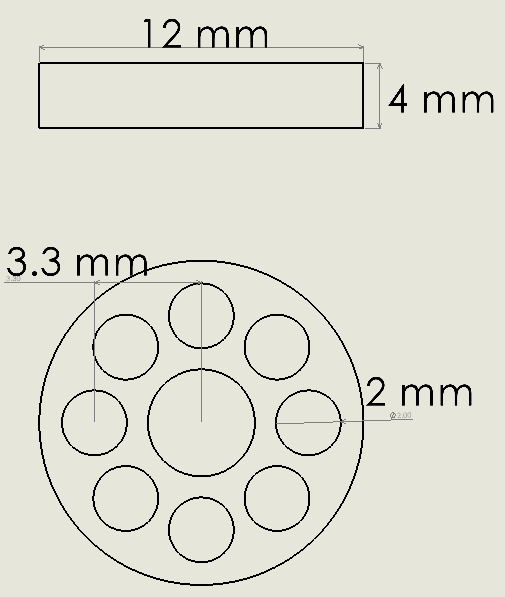
\includegraphics[scale=0.3]{pic/setu.PNG}
  \caption{開発した器具}
  \label{fig:setu}
\end{figure}
また空圧筋として動作させるための器具を作製した(図\ref{fig:kuro}).
作製手順を以下に示す.
\begin{enumerate}
  \item 送気用のポリウレタンチューブを約5 cm切る
  \item 作製した空圧筋を図\ref{fig:kuro}に約1 cm差し込む
  \item 重なった部分をPEラインで結び,強く締結する
  \item 締結下部分に接着剤を塗布し糸が緩まないようにする
  \item Oリングを任意の数はめ込む
  \item 図\ref{fig:kuro}を他方に挿入して同様にPEラインで締結し,接着剤を塗布する
  \item ポリウレタンチューブを図\ref{fig:kuro}にはめ,接着剤を塗布し完成する
\end{enumerate}
\begin{figure}[h]
  \centering  % 図全体を中央に配置
  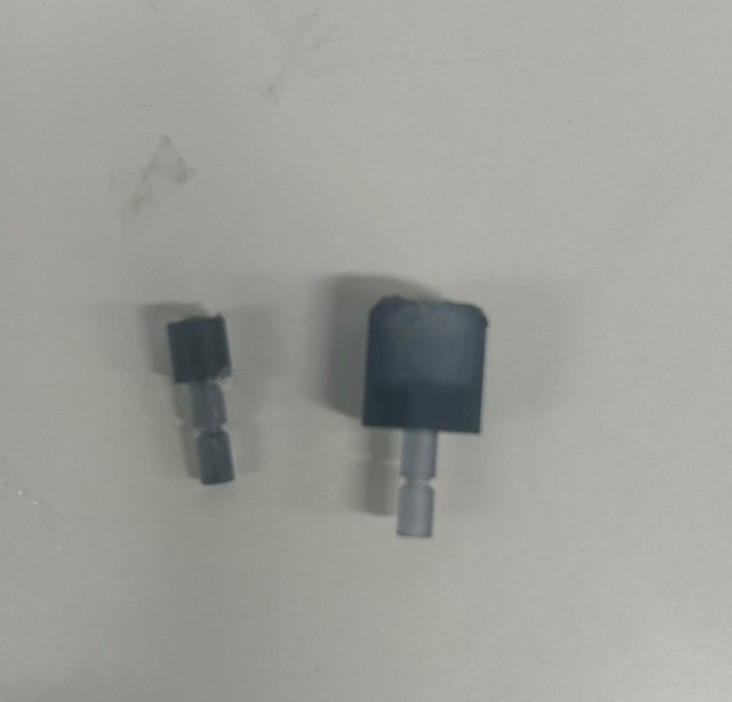
\includegraphics[scale=0.3]{pic/S__157270018.jpg}
  \caption{開発した器具}
  \label{fig:kuro}
\end{figure}





\subsection{作製方法1}
作製方法1では前章と同様,鉄棒の周りに糸を張り液体ゴムに漬けることで作製を行った.
作製した人工筋肉を図\ref{fig:18},\ref{fig:19}に示す.
内径が小さくなったことで図\ref{fig:18}から見て取れるように経糸同士の間隔が狭くなり,互いにくっついてしまう現象が生じた.
これによりゴム膜の幅に偏りが生じ,空圧印加時に破裂しやすくなってしまった.
\begin{figure}[!h]
  \centering  % 図全体を中央に配置
  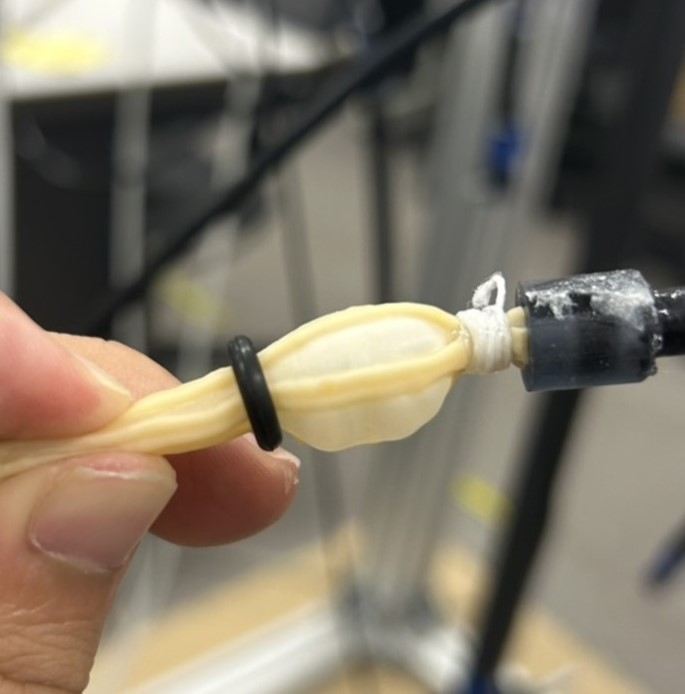
\includegraphics[scale=0.3]{pic/17.jpg}
  \caption{作製方法1}
  \label{fig:18}
\end{figure}
\begin{figure}[!h]
  \centering  % 図全体を中央に配置
  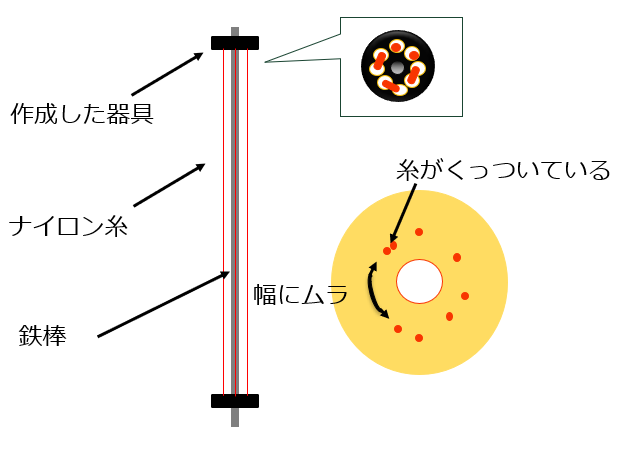
\includegraphics[scale=0.5]{pic/18.PNG}
  \caption{作製方法1}
  \label{fig:19}
\end{figure}
\newpage
\subsection{作製方法2}
作製方法2では糸同士の間隔が一定になるように図\ref{fig:20}のように鉄棒と縦糸の間隔を近づけて作製を行った.作製手順を以下と図\ref{fig:21}に示す.
\begin{enumerate}
  \item まず初めに器具を取り付ける
  \item ナイロン糸を器具に通す
  \item PEラインを使いナイロン糸を鉄棒に押し付ける
  \item 凝固液に約5秒浸して取り出す
  \item 凝固液の水滴がなくなるまでドライヤーで乾かす
  \item 液体ゴムに約5秒浸して取り出す
  \item ドライヤーで凝固液の水滴がなくなるまで乾かす
  \item 凝固液に約5秒浸して取り出す
  \item 取り出した鉄棒をゴム膜の外側のいろが白色から肌色になるまでドライヤーで乾かす
  \item 3時間程部屋で乾かしたら鉄棒からゴム膜をとる
\end{enumerate}
\begin{figure}[h]
  \centering  % 図全体を中央に配置
  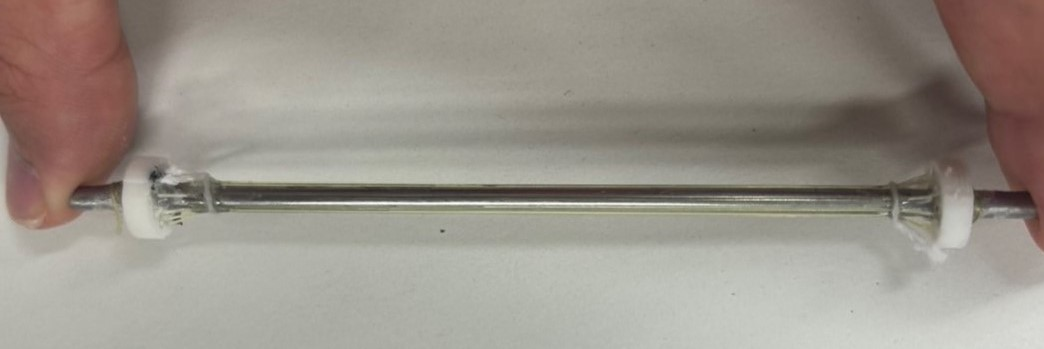
\includegraphics[scale=0.2]{pic/19.jpg}
  \caption{作製方法2}
  \label{fig:20}
\end{figure}
\vspace{30mm}
\begin{figure}[h]
  \centering  % 図全体を中央に配置
  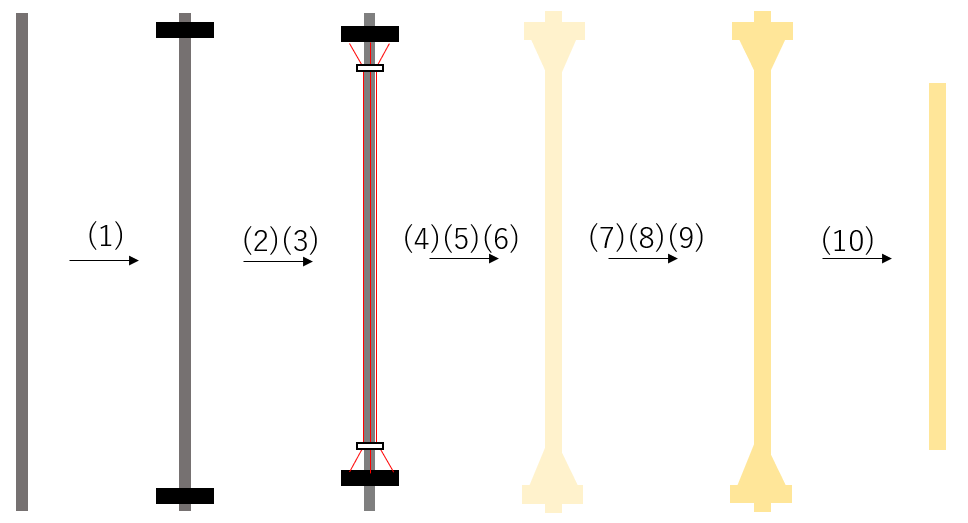
\includegraphics[scale=0.4]{pic/19.PNG}
  \caption{作製手順}
  \label{fig:21}
\end{figure}

縦糸がくっつく現象は解決したものの,ゴム部内面に隙間がなくなった結果,図\ref{fig:22},\ref{fig:23}のように内面側から縦糸が抜けてしまう問題が新たに発生し,軸方向への膨張を抑制することができなかった.
\begin{figure}[ht]
  \centering  % 図全体を中央に配置
  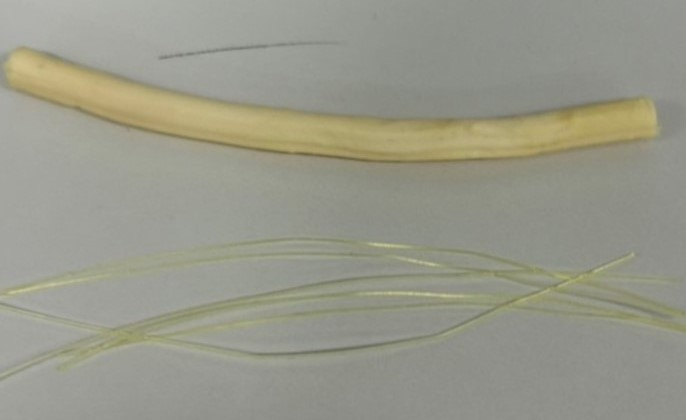
\includegraphics[scale=0.3]{pic/20.jpg}
  \caption{作製方法2}
  \label{fig:22}
\end{figure}
\begin{figure}[ht]
  \centering  % 図全体を中央に配置
  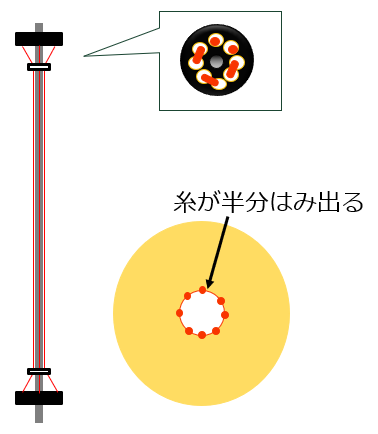
\includegraphics[scale=0.5]{pic/21.PNG}
  \caption{作製方法2}
  \label{fig:23}
\end{figure}
\newpage
\subsection{作製方法3}
作製方法3では糸が簡単に取れなくなるように鉄棒にゴム膜を作り,その上に糸を押し付けて固定し作製を行った.
作製手順を以下と図\ref{fig:24}に示す.
\begin{enumerate}
  \item 凝固液に約5秒浸して取り出す
  \item 凝固液の水滴がなくなるまでドライヤーで乾かす
  \item 液体ゴムに約2秒浸して取り出す
  \item 凝固液に約5秒浸して取り出す
  \item 凝固液の水滴がなくなるまでドライヤーで乾かす
  \item 液体ゴムに約2秒浸して取り出す
  \item 凝固液に約5秒浸して取り出す
  \item 凝固液の水滴がなくなるまでドライヤーで乾かす
  \item 器具を取り付ける
  \item ナイロン糸を器具に通す
  \item PEラインを使いナイロン糸をゴム膜に押し付ける
  \item 凝固液に約5秒浸して取り出す
  \item 凝固液の水滴がなくなるまでドライヤーで乾かす
  \item 液体ゴムに約5秒浸して取り出す
  \item ドライヤーで凝固液の水滴がなくなるまで乾かす
  \item 凝固液に約5秒浸して取り出す
  \item 取り出した鉄棒をゴム膜の外側のいろが白色から肌色になるまでドライヤーで乾かす
  \item 3時間程部屋で乾かしたら鉄棒からゴム膜をとる
\end{enumerate}
\begin{figure}[h]
  \centering  % 図全体を中央に配置
  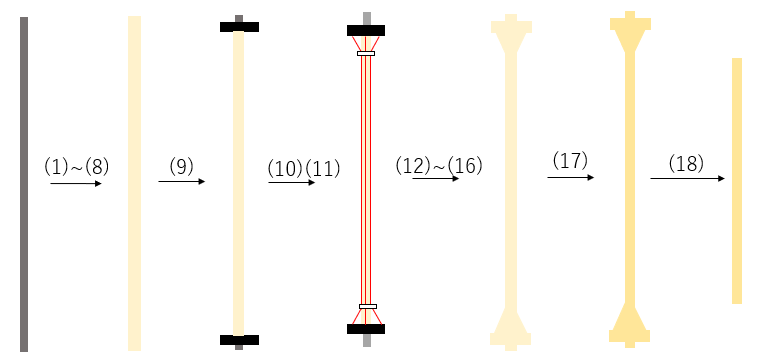
\includegraphics[scale=0.4]{pic/2211.PNG}
  \caption{作製手順}
  \label{fig:24}
\end{figure}
内面側から糸が抜ける問題は改善したものも糸がある場所で図\ref{fig:25}のようにゴム膜が2つの層に分かれてしまい,強度が低下し破裂が生じ
てしまった.
\begin{figure}[t]
  \centering  % 図全体を中央に配置
  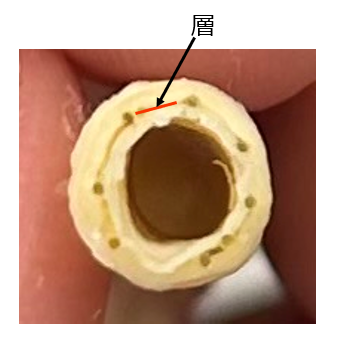
\includegraphics[scale=0.8]{pic/24.PNG}
  \caption{作製方法3}
  \label{fig:25}
\end{figure}
\subsection{作製方法4}
糸を入れてないときは層ができなかったので,糸にゴムをコーティングすれば糸がある場所に層ができないと考えた.
図\ref{fig:26}に糸にゴムをコーティングする方法を示す.必要な物品は以下の通りである.
\begin{itemize}
  \item REGITEX 液体ゴム(前加硫ラッテクス) メーカー:有限会社 ハイラテック
  \item PC-518用 凝固液
  \item 作製した器具
  \item アーマードF+pro 0.06号
  \item 綿 手縫い糸
  \item オーブントースター CF-AC121
  \item 作製した器具
\end{itemize}
以下,作成手順である
\begin{enumerate}
  \item 糸を図\ref{fig:26}のように巻きつける
  \item 凝固液に約5秒浸して取り出す
  \item 凝固液の水滴がなくなるまでドライヤーで乾かす
  \item 液体ゴムに約10秒浸して取り出す
  \item 凝固液に約5秒浸して取り出す
  \item オーブントースターで80度で10分乾かす
\end{enumerate}

この方法で作製した糸を用いて作製方法3と同様な方法で作製を行った.また今回からオーブンを使用して乾燥を行った.
図\ref{fig:27}からみて分かるように糸をゴムでコーティングしても層ができる現象は改善されなかった.
\begin{figure}[h]
  \centering  % 図全体を中央に配置
  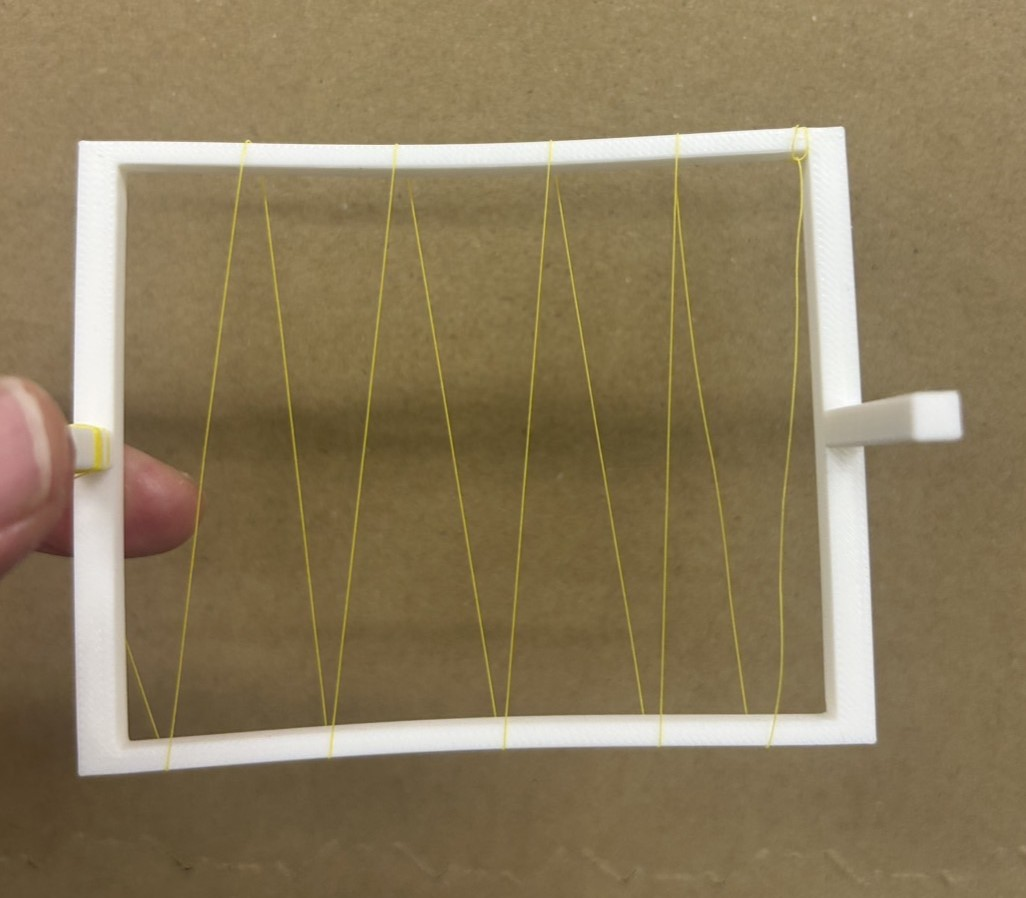
\includegraphics[scale=0.2]{pic/25.jpg}
  \caption{コーティング方法}
  \label{fig:26}
\end{figure}
\begin{figure}[h]
  \centering  % 図全体を中央に配置
  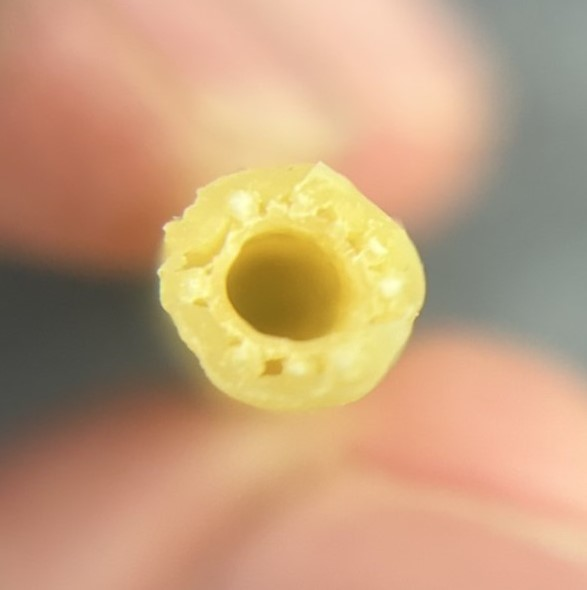
\includegraphics[scale=0.4]{pic/26.jpg}
  \caption{作製方法3}
  \label{fig:27}
\end{figure}
\subsection{作製方法5}
作製方法5ではゴムが2層になる問題を回避するために,作製方法1と同様1度にゴム膜を形成する方法に戻した.
また糸がくっつく問題を回避するために,縦糸にテンションをかけるネジを用いた器具を開発した.
開発した器具の使用方法を図\ref{fig:mawa}に示す.
\begin{figure}[h]
  \centering  % 図全体を中央に配置
  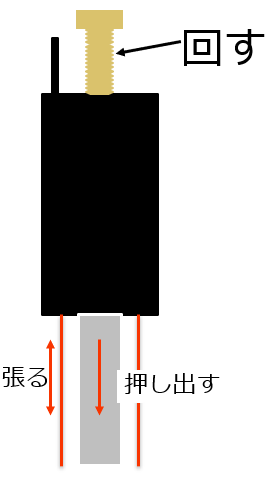
\includegraphics[scale=0.4]{pic/mawa.PNG}
  \caption{使用方法}
  \label{fig:mawa}
\end{figure}

作製方法を以下と図\ref{fig:ten}に示す.
\begin{enumerate}
  \item 器具を鉄棒に取り付ける
  \item 器具に糸を通しネジを回すことで糸にテンションをかける
  \item 凝固液に約5秒浸して取り出す
  \item 凝固液の水滴がなくなるまでドライヤーで乾かす
  \item 液体ゴムに約10秒浸して取り出す
  \item 凝固液に約5秒浸して取り出す
  \item 取り出した鉄棒をゴム膜の外側のいろが白色から肌色になるまでドライヤーで乾かす
 \item 3時間程部屋で乾かしたら鉄棒からゴム膜をとる
\end{enumerate}
\begin{figure}[h]
  \centering  % 図全体を中央に配置
  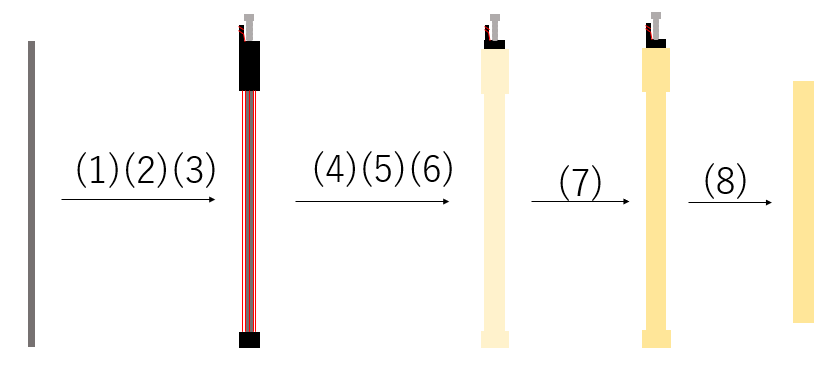
\includegraphics[scale=0.4]{pic/ten.PNG}
  \caption{使用方法}
  \label{fig:ten}
\end{figure}
作製方法4ではオーブンで乾かすことによりゴム膜を硬くしていたが,硬くなることによって膨張が起きにくくなっていたので部屋でゆっくりと乾燥させる方式に戻した.
作製した人工筋肉は図\ref{fig:2sou},\ref{fig:kutu}のように糸のくっつきおよび2層化の問題は生じなかった.また印加圧力によって空圧筋として動作することが確認した.
\begin{figure}[h]
  \centering  % 図全体を中央に配置
  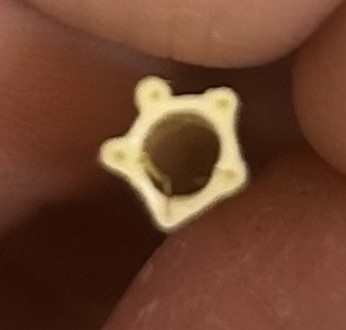
\includegraphics[scale=0.4]{pic/2sou.jpg}
  \caption{断面}
  \label{fig:2sou}
\end{figure}
\begin{figure}[h]
  \centering  % 図全体を中央に配置
  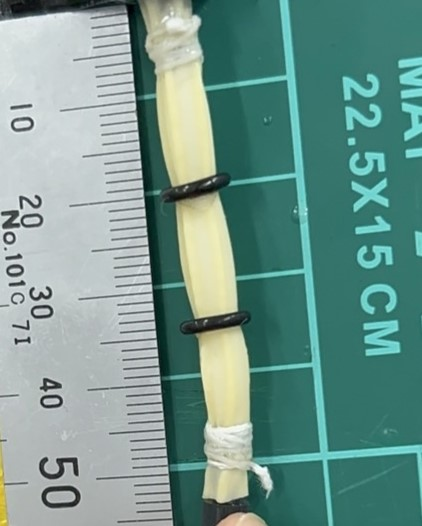
\includegraphics[scale=0.4]{pic/kutu.jpg}
  \caption{糸の配置}
  \label{fig:kutu}
\end{figure}

 


